\chapter{System Analysis and Requirements}
\label{chap:requirements}

This chapter defines the precise specifications for the TEKUTOKO platform, translating the research objectives into a concrete set of functional and non-functional requirements. It serves as the foundational blueprint for the subsequent design, implementation, and evaluation phases, ensuring that the final product aligns with the project's goals.

\section{Requirements Gathering Methodology}
\label{sec:req-gathering}
The requirements for the TEKUTOKO platform were gathered and refined through a multi-faceted approach to ensure comprehensive coverage of user needs and technical feasibility:
\begin{enumerate}
    \item \textbf{Literature Review:} The analysis of academic papers on e-learning, gamification, and online proctoring (as detailed in Chapter \ref{chap:lit-review}) helped identify established best practices and core pedagogical needs.
    \item \textbf{Competitive Analysis:} A thorough examination of existing platforms (Kahoot!, Quizlet, Google Classroom, and specialized proctoring tools) was conducted to determine market standards, identify common features, and pinpoint opportunities for innovation.
    \item \textbf{Stakeholder Needs Analysis:} Potential end-users, including educators and students, were consulted to understand their primary pain points with current systems. Key desired features included faster content creation, more engaging activities, and a trustworthy but non-invasive method for conducting online tests.
    \item \textbf{Prototyping:} Low-fidelity mockups and user flow diagrams were created to visualize core concepts and gather early feedback, ensuring the proposed system would be intuitive and user-friendly.
\end{enumerate}

\section{Functional Requirements}
\label{sec:func-req}
Functional requirements describe the specific behaviors, features, and functions the system must perform. They are detailed in Table \ref{tab:func-req}.

\begin{longtable}{l l p{8.5cm}}
\caption{Functional Requirements} \label{tab:func-req} \\
\toprule
\textbf{ID} & \textbf{Category} & \textbf{Requirement Description} \\
\midrule
\endfirsthead
\multicolumn{3}{c}%
{{\bfseries Table \thetable\ continued from previous page}} \\
\toprule
\textbf{ID} & \textbf{Category} & \textbf{Requirement Description} \\
\midrule
\endhead
\bottomrule
\endfoot
\bottomrule
\endlastfoot

% User Management
\multicolumn{3}{l}{\textbf{FR1: User \& Profile Management}} \\
\midrule
FR1.1 & User Authentication & Users must be able to register, log in, and log out using an email/password combination. The system must use JWT for session management. \\
FR1.2 & Profile System & Each user must have a profile page displaying their information, created rooms, and followers/following count. \\
FR1.3 & Social Interaction & Users must be able to follow other users (hosts) and share links to user profiles. \\
\midrule

% Room Management
\multicolumn{3}{l}{\textbf{FR2: Room Creation \& Management (Host)}} \\
\midrule
FR2.1 & Room Type Selection & Hosts must be able to create two distinct types of rooms: a gamified \textbf{"Quiz Room"} or a secure \textbf{"Test Room"}. \\
FR2.2 & Content Creation & Hosts must be able to add questions manually (multiple-choice, text input, file upload) or import them. \\
FR2.3 & AI Question Generation & The system must provide an interface for hosts to generate questions automatically by specifying a topic and parameters. \\
FR2.4 & DOCX Import & The system must allow hosts to upload a `.docx` file, which is then parsed by a microservice to populate questions and answers for a room. \\
FR2.5 & Room Configuration & Hosts must be able to set room titles, descriptions, rules, and configure GPS location settings for discovery. \\
FR2.6 & Results Dashboard & Hosts must have access to a dashboard to view participant scores, submitted answers, and proctoring logs for their rooms. \\
\midrule

% Participant Interaction
\multicolumn{3}{l}{\textbf{FR3: Participant Interaction}} \\
\midrule
FR3.1 & Room Participation & Users must be able to join a room using a unique code or by clicking a direct link. \\
FR3.2 & Answering Questions & Participants must be able to view questions and submit their answers within the defined format for each room type. \\
FR3.3 & Real-time Updates & In Quiz Rooms, the leaderboard and scores must update in near real-time. \\
\midrule

% Gamification
\multicolumn{3}{l}{\textbf{FR4: Gamification \& Rewards}} \\
\midrule
FR4.1 & Leaderboard & Quiz Rooms must feature a live leaderboard displaying participant scores and rankings. \\
FR4.2 & Reward Configuration & Hosts must be able to create digital rewards (vouchers, tickets) for completing a Quiz Room. \\
FR4.3 & Reward Issuance & The system must automatically issue a unique QR code for the reward to participants who meet the completion criteria. \\
FR4.4 & QR Code Verification & The system must provide a mechanism for hosts to scan a participant's QR code to validate and redeem the reward, marking it as used. \\
\midrule

% Proctoring
\multicolumn{3}{l}{\textbf{FR5: Anti-Cheating / Proctoring (Test Room)}} \\
\midrule
FR5.1 & Tab-Switching Detection & The system must detect when a participant navigates away from the test tab/window and log this event. \\
FR5.2 & Inactivity Monitoring & The system must monitor for prolonged periods of user inactivity during a test and flag it as a potential issue. \\
FR5.3 & Proctoring Logs & All detected suspicious events must be logged with timestamps and made available to the host. \\
\midrule

% Discovery
\multicolumn{3}{l}{\textbf{FR6: Discovery \& Community}} \\
\midrule
FR6.1 & Room Discovery & The system must provide a discovery page with search functionality and a "Nearby" feature that uses the device's GPS to find local rooms. \\
FR6.2 & Popularity Ranking & The discovery page should feature and suggest rooms based on popularity metrics (e.g., number of participants, host followers). \\
\midrule

% Admin Panel
\multicolumn{3}{l}{\textbf{FR7: Administrator Panel}} \\
\midrule
FR7.1 & System Dashboard & An admin panel must exist to display system-wide statistics (e.g., total users, active rooms). \\
FR7.2 & Management & Administrators must be able to manage users and rooms (e.g., delete inappropriate content, resolve user reports). \\
\end{longtable}

\section{Non-Functional Requirements}
\label{sec:non-func-req}
Non-functional requirements define the quality attributes, performance standards, and constraints of the system, detailed in Table \ref{tab:non-func-req}.

\begin{table}[htbp]
\centering
\caption{Non-Functional Requirements}
\label{tab:non-func-req}
\begin{tabular}{l l p{8.5cm}}
\toprule
\textbf{ID} & \textbf{Category} & \textbf{Requirement Description} \\
\midrule
\multicolumn{3}{l}{\textbf{NFR1: Performance}} \\
\midrule
NFR1.1 & API Response Time & 95\% of API requests under normal load should complete in under 500ms. AI generation requests are exempt but should not exceed 20 seconds. \\
NFR1.2 & Concurrency & The system must support at least 100 concurrent users in a single real-time quiz room without significant performance degradation. \\
\midrule
\multicolumn{3}{l}{\textbf{NFR2: Scalability}} \\
\midrule
NFR2.1 & Horizontal Scaling & The backend architecture must be stateless and allow for horizontal scaling by adding more server instances behind a load balancer. \\
NFR2.2 & Microservice Independence & The Python microservice must be independently scalable from the main Node.js backend. \\
\midrule
\multicolumn{3}{l}{\textbf{NFR3: Usability}} \\
\midrule
NFR3.1 & User Interface & The UI must be intuitive, responsive across devices (desktop, tablet, mobile), and adhere to modern design principles. \\
NFR3.2 & Accessibility & The platform should follow Web Content Accessibility Guidelines (WCAG) 2.1 Level A standards. \\
\midrule
\multicolumn{3}{l}{\textbf{NFR4: Security}} \\
\midrule
NFR4.1 & Data Transmission & All communication between the client and server must be encrypted using HTTPS/TLS. \\
NFR4.2 & Authentication & User authentication must be secured using JSON Web Tokens (JWT). Passwords must be securely hashed (e.g., using bcrypt) before storage. \\
NFR4.3 & Input Validation & The system must validate and sanitize all user inputs on both the client and server sides to prevent XSS, SQL Injection, and other vulnerabilities. \\
\midrule
\multicolumn{3}{l}{\textbf{NFR5: Reliability \& Maintainability}} \\
\midrule
NFR5.1 & Uptime & The system should maintain a service uptime of at least 99.5\%. \\
NFR5.2 & Modularity & The codebase must be well-documented and organized into logical, loosely coupled modules to facilitate maintenance and future development. \\
\bottomrule
\end{tabular}
\end{table}

\FloatBarrier
\section{Use Case Analysis}
\label{sec:use-case}

\subsection{System Actors}
\begin{itemize}
    \item \textbf{Participant (User):} A registered user who joins rooms, participates in quizzes/tests, discovers content, and interacts with social features.
    \item \textbf{Host (Educator):} A user with elevated privileges to create, manage, and monitor game rooms and test rooms.
    \item \textbf{Administrator:} A privileged user responsible for overseeing the entire platform, managing content, and viewing system-wide analytics.
\end{itemize}

\subsection{Use Case Diagram}
Figure \ref{fig:use-case-diagram} illustrates the primary interactions between the actors and the TEKUTOKO system.

\begin{figure}[htbp]
\centering
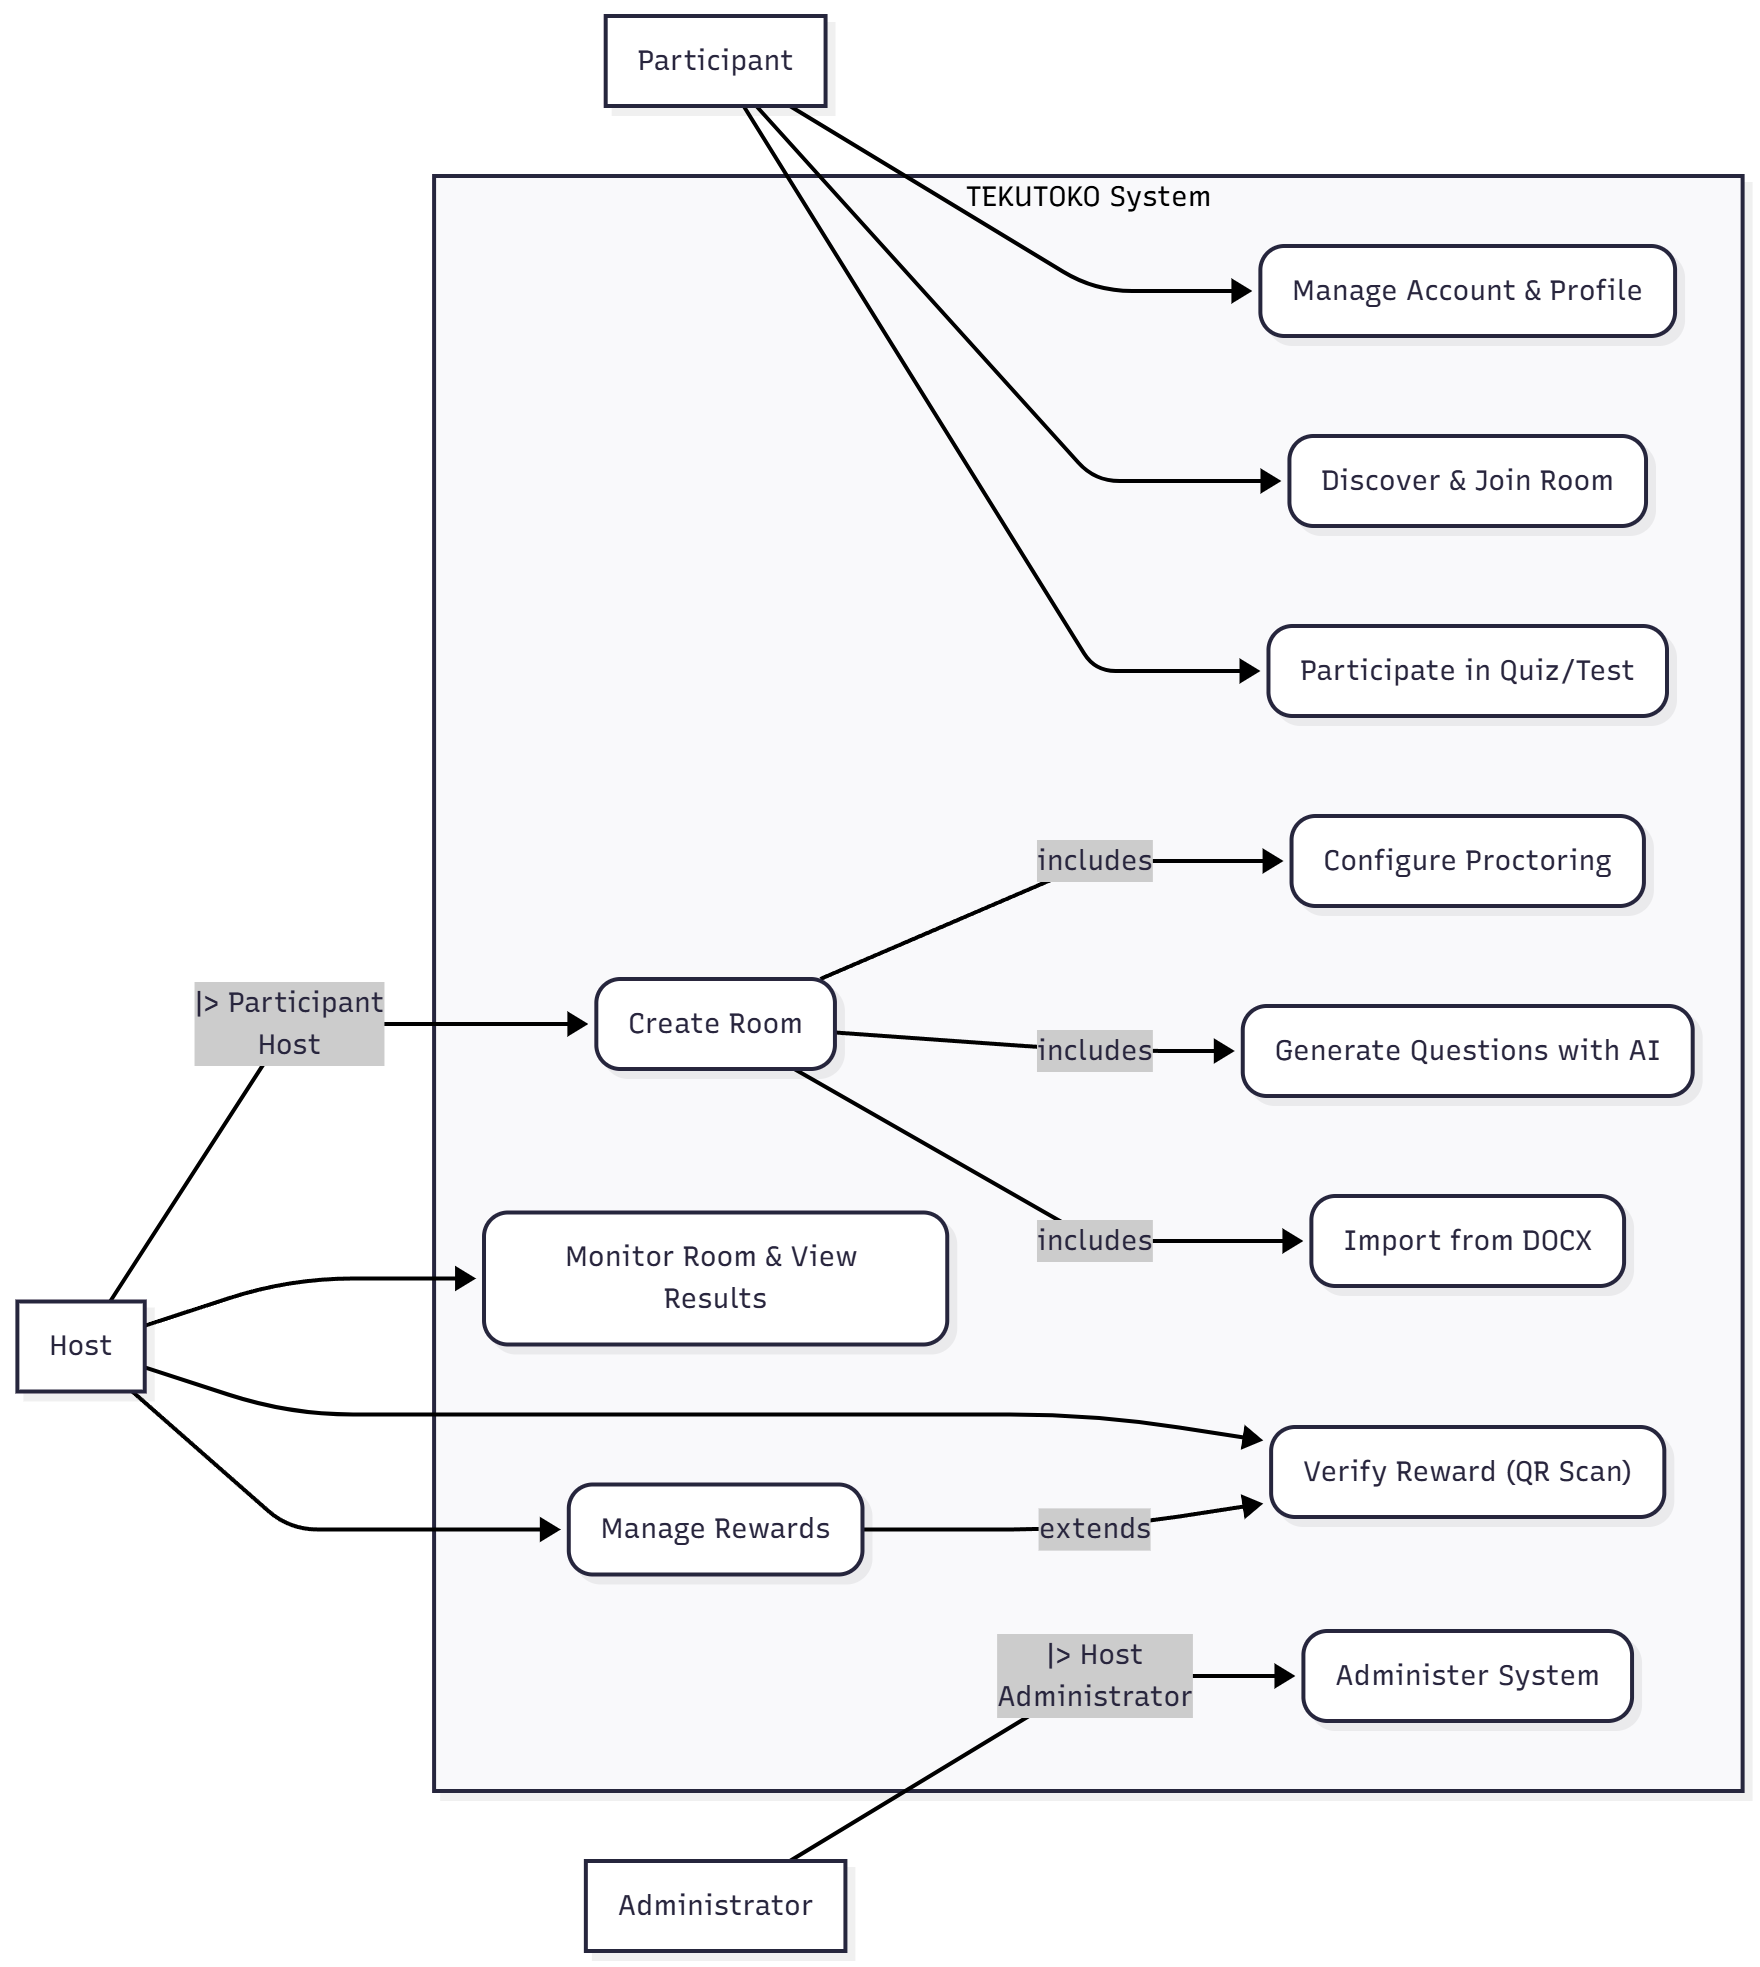
\includegraphics[width=0.9\textwidth]{figures/use-case-diagram.png}
\caption{Use Case Diagram for the TEKUTOKO System}
\label{fig:use-case-diagram}
\end{figure}

\subsection{Detailed Use Case Specifications}

\subsubsection{Use Case 1: Create a Proctored Test from a DOCX file}
\begin{itemize}
    \item \textbf{Actor:} Host (Educator)
    \item \textbf{Description:} The Host creates a secure online test by uploading a pre-formatted document and enabling anti-cheating features.
    \item \textbf{Preconditions:} The Host is logged into the system. The Host has a `.docx` file containing questions and marked answers.
    \item \textbf{Flow:}
    \begin{enumerate}
        \item Host selects "Create Room" and chooses the "Test Room" type.
        \item Host enters test details (title, instructions, duration).
        \item Host selects the "Import from DOCX" option and uploads the file.
        \item The system sends the file to the Python microservice for parsing.
        \item The microservice returns a structured JSON of questions and answers, which populates the test configuration.
        \item Host navigates to the "Proctoring" tab and enables "Tab-Switching Detection" and "Inactivity Monitoring".
        \item Host saves the test. The system generates a unique URL and join code for the test.
    \end{enumerate}
    \item \textbf{Postconditions:} A secure test room is created and is ready for participants to join.
\end{itemize}

\vspace{1cm}

\subsubsection{Use Case 2: Verify a Reward Voucher}
\begin{itemize}
    \item \textbf{Actor:} Host
    \item \textbf{Description:} A participant who won a reward in a quiz presents their QR code to the Host for verification and redemption.
    \item \textbf{Preconditions:} The Host is logged in. A participant has a valid, unredeemed reward QR code.
    \item \textbf{Flow:}
    \begin{enumerate}
        \item Participant displays the QR code on their device.
        \item Host navigates to the "Verify Voucher" section of the TEKUTOKO application.
        \item Host uses their device's camera to scan the participant's QR code.
        \item The system sends the scanned data to the backend for verification.
        \item The backend checks the voucher's validity and redemption status in the database.
        \item \textbf{If valid:} The system displays a "Success" message to the Host and marks the voucher as "redeemed" in the database.
        \item \textbf{If invalid or already used:} The system displays an "Error" or "Already Redeemed" message.
    \end{enumerate}
    \item \textbf{Postconditions:} The reward voucher is successfully redeemed and can no longer be used.
\end{itemize}